\subsubsection{Pruning Analysis}


Consider the amount of pruning that can be obtained when using BAB. 
Next, we provide a worst-case and best-case analysis of the amount of pruning obtained when using BAB, when applied to deterministic games. To put our results in context, we remind the reader that in a balanced game tree with a branching factor $b$ and depth $d$, Alpha Beta will generate $O(b^d)$ in the worst case and $O(b^{d/2})$ in the best case~\cite{knuth1975analysis}. 
\begin{theorem}
If $\epsilon < \vmax - \vmin$, then for any input and-or tree, there is a worst-case assignment of values to the leaves so that BAB going left to right develops the full tree.
\label{the:worst}
\end{theorem}
\begin{proof}
First, we determine the assignment of values to the leaves by recursively assigning values to nodes in a top down fashion as follows.

\begin{itemize}
  \item For a max node $n$ assigned to value $v$, we assign the $b(n)-1$ first children of $n$ the value $\vmin$, and assign the $b(n)$th child value $v$.
  \item For a min node $n$ assigned to value $v$, we assign the $b(n)-1$ first children of $n$ the value $\vmax$, and assign the $b(n)$th child value $v$.
  \item For a leaf node assigned to value $v$, we just assign the value $v$.
  \item The above rules define the heredity part of the recursion, for the starting case: it suffices to assign the root to any value strictly between $\vmin$ and $\vmax$.
\end{itemize}

The following facts establish by induction that every node on the tree gets the value assigned in the construction.
\begin{itemize}
  \item A leaf node value is the same value assigned to it in the construction.  
  \item Assuming node children values are the assigned values in the construction, max node $n$ children values are $\vmin$ for the $b(n)-1$ first children and $v$ for the $b(n)$th child. Since $v \geq \vmin$, the value of $n$ must be $v$.
    \item Assuming node children values are the assigned values in the construction, min node $n$ children values are $\vmax$ for the $b(n)-1$ first children and $v$ for the $b(n)$th child. Since $v \leq \vmax$, the value of $n$ must be $v$.
\end{itemize}

During the algorithm for each partially expanded node the $\alpha$ and $\beta$ values are $\vmin$ and $\vmax$ respectively.
\begin{itemize}
  \item A max node $n$ updates its $\alpha$ value after each child. Since the assigned value of the $b(n)-1$ first children is $\vmin$, the value of $\alpha$ remains $\vmin$.
  \item A min node $n$ updates its $\beta$ value after each child. Since the assigned value of the $b(n)-1$ first children is $\vmax$, the value of $\beta$ remains $\vmax$.
\end{itemize}
The algorithm commits pruning if $\beta - \alpha \leq \epsilon$. Because $\alpha = \vmin$ and $\beta = \vmax$ for every partially expanded node, pruning will be committed if $\vmax - \vmin \leq \epsilon$. However, $\epsilon < \vmax - \vmin$ and hence no pruning ever occurs
\end{proof}


\begin{theorem}
If the value of all terminal states is within the range $[\vmin+\epsilon, \vmax-\epsilon]$, then in a balanced tree with depth $d$ and branching factor $b$, the best-case pruning of BAB will not prune at least $O(b^{d/2})$ nodes. 
\label{the:best}
\end{theorem}
\begin{proof}
For our proof, we define recursively the following types three types of nodes:

\begin{itemize}
\item \textbf{Type 1.} The root is a type 1 node, and the first child of every type 1 node is also a type 1 node. 
\item \textbf{Type 2.} All the children of a type 1 node except the first one are type 2 nodes. The first child of a type 2 node is a type 3 node. 
\item \textbf{Type 3.} The first child of a type 3 node is also a type 3 node. All other children of a type 3 node are type 2 nodes. 
\end{itemize}
\end{proof}

TODO: Provide invariants over the types

%Like Alpha-Beta and *-Minimax, in the worst case we still may need to generate all nodes in the game tree before halting, as long as $\epsilon<\vmax-\vmin$.  Such a worst case occurs, for example, when the children of MAX nodes all lead to $\vmin$ except one node and the children of MIN nodes all lead to $\vmax$ except one node, and this individual nodes are always generated last. 
%In the best case, however, significant pruning can be achieved. We conjecture that the best case cannot be better than that of Alpha Beta, except for the case where $\epsilon=\vmax-\vmin$, in which only a single branch in the game tree will be expanded, but the resulting value is not helpful. 
% This is in contrast to Alpha-Beta's worst case, which is exponential in half the depth of the game tree.




\begin{figure}
	\centering
    \hfill\subfloat[$\epsilon=2$]{
  \begin{tikzpicture}[yscale=-1]
    \node[maxnode] (s0)  at (1.5, 0) {};
%    \node[maxnode] (s0)  at (1.5, 0) {$\pess=8$\\$\opti=10$};
    \node[minnode] (s1) at (1.0, 1) {$7$};
    \node[minnode] (s2) at (2.0, 1) {};
    \node[maxnode] (s3) at (1.5, 2) {};
    \node[maxnode] (s4) at (2.5, 2) {$10$};
    \node[minnode] (s5) at (1.0, 3) {$8$};
    \node[minnode] (s6) at (2.0, 3) {};
    \node[infobox] (i0) at ($(s0) + (-0.5, 0)$) {$A$};
    \node[infobox] (i2) at ($(s2) + (0.5, 0)$) {$B$};
    \node[infobox] (i3) at ($(s3) + (-0.5, 0)$) {$C$};
    \node[infobox] (i4) at ($(s4) + (0.5, 0)$) {$D$};
    \node[infobox] (i6) at ($(s6) + (0.5, 0)$) {$E$};
    \node[infobox] (i0ul) at ($(s0) + (+0.9, 0)$) {$\pess=8$\\$\opti=10$};
    
    \draw[->] (s0)  -- (s1);
    \draw[->] (s0)  -- (s2);
    \draw[->] (s2)  -- (s3);
    \draw[->] (s2)  -- (s4);
    \draw[->] (s3)  -- (s5);
    \draw[->] (s3)  -- (s6);
    \draw[thick,draw=red] ($(s3) + (0.35, 0.4)$) -- ($(s3) + (0.15, 0.6)$);
  \end{tikzpicture}}\hfill
  \subfloat[$\epsilon=1$]{
  \begin{tikzpicture}[yscale=-1]
    \node[maxnode] (s0)  at (1.5, 0) {};
%    \node[maxnode] (s0)  at (1.5, 0) {$\pess=8$\\$\opti=10$};
    \node[minnode] (s1) at (1.0, 1) {$7$};
    \node[minnode] (s2) at (2.0, 1) {};
    \node[maxnode] (s3) at (1.5, 2) {};
    \node[maxnode] (s4) at (2.5, 2) {};
    \node[minnode] (s5) at (1.0, 3) {$8$};
    \node[minnode] (s6) at (2.0, 3) {$8$};
    \node[infobox] (i0) at ($(s0) + (-0.5, 0)$) {$A$};
    \node[infobox] (i2) at ($(s2) + (0.5, 0)$) {$B$};
    \node[infobox] (i3) at ($(s3) + (-0.5, 0)$) {$C$};
    \node[infobox] (i4) at ($(s4) + (0.5, 0)$) {$D$};
    \node[infobox] (i6) at ($(s6) + (0.5, 0)$) {$E$};
    \node[infobox] (i0ul) at ($(s0) + (+0.9, 0)$) {$\pess=7$\\$\opti=8$};
    
    \draw[->] (s0)  -- (s1);
    \draw[->] (s0)  -- (s2);
    \draw[->] (s2)  -- (s3);
    \draw[->] (s2)  -- (s4);
    \draw[->] (s3)  -- (s5);
    \draw[->] (s3)  -- (s6);
    \draw[thick,draw=red] ($(s2) + (0.35, 0.4)$) -- ($(s2) + (0.15, 0.6)$);
  \end{tikzpicture}}\hfill~
%	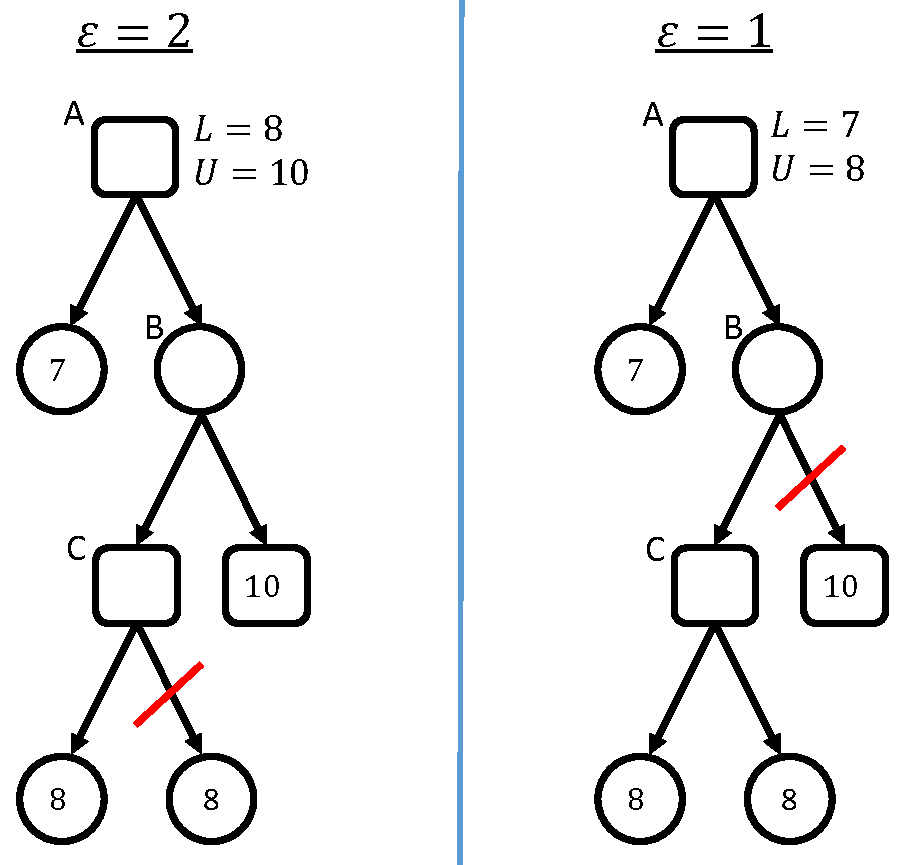
\includegraphics[width=0.6\columnwidth]{Figures/cropped_example_different_e.pdf}
	\caption{Example of BAB pruning with different suboptimality values. Depending on the relative size of the subtrees rooted in $D$ and $E$, $\epsilon = 2$ may lead to more or less pruning than $\epsilon = 1$.}
	\label{fig:bab-prune}
    \vspace{-0.5cm}
\end{figure}


Interestingly, in some case, increasing $\epsilon$ may actually result in fewer nodes begin pruning. For example, consider the case depicted in 
Figure \ref{fig:bab-prune}. The right tree represent an example of BAB with $\epsilon = 1$ and the left one represent BAB with $\epsilon = 2$. In both cases $\vmin = 0$ and $\vmax = 10$. In both cases, after node $A$ explored the left child its $\alpha = 7$ and $\beta = 10$. These values transmitted down to $B$ and from there to $C$. After $C$ explored the left child $\alpha = 8$ and $\beta = 10$. In this point, the left tree prune the right branch and the values that return to $B$ are $(8,10)$, node $B$ update $\beta$ value to $10$ and explore the right child. In the right tree, the right child of $C$ does not get pruned and the values that return to $B$ are $(8,8)$, $B$ update $\beta$ value to $8$ and the right child get pruned. Although these two examples explored the same amount of nodes, the branch of the right child of $B$ and the branch of the right child of $C$ could contain large sub-trees and hence a greater $\epsilon$ value might explore less, more or equal amount of nodes. 


While the example in Figure~\ref{fig:bab-prune} shows that increasing $\epsilon$ may cause fewer nodes to be pruned, we verify experimentally  this usually do not occur in practice, and indeed increasing $\epsilon$ results in a faster search. %.However, in some special cases, BAB with $\epsilon_2$ actually prunes fewer nodes than BAB with $\epsilon_1$. 

%---------------------------------------------------------
%---------------------------------------------------------